\documentclass{article}
\usepackage[utf8]{inputenc}
\usepackage{imakeidx}
\usepackage[italian]{babel}
\usepackage{graphicx}
\usepackage[T1]{fontenc}
\makeindex
\usepackage{float}
%\graphicspath{}
\title{Sintetizzatore di Frequenza}
\author{William Perri 4427140 }
\setlength{\parskip}{1em}
\renewcommand{\baselinestretch}{1}
%\DeclareGraphicsExtensions{.jpeg,.png}
\date{20/06/2020}

\begin{document}

\maketitle
Insegnamento di LABORATORIO DI ELETTRONICA A.A. 2019/20

\newpage
\tableofcontents
\newpage
\section{Introduzione}
\paragraph{Lo scopo del progetto consiste nel realizzare un sintetizzatore di frequenza basato su PLL (Phase Locked Loop).
Un PLL è composto da un rivelatore di fase, un filtro passa-basso ed un VCO (Voltage Controlled Oscillator).}
\paragraph{ Il progetto verrà dapprima simulato mediante software di simulazione ed in seguito realizzato in parte su breadboard ed in parte su una FPGA (Field Programmable Gate Array) Cyclone II, programmata mediante il software Quartus II sulla base del progetto realizzato su Digital Electronic Deeds.}


\newpage
\section{Descrizione del Progetto}

\paragraph{Come già detto nel capitolo precedente, il nostro sintetizzatore si baserà su un PLL il cui schema a blocchi è il seguente:\\ }

~\begin{figure}[!h]%Schema a blocchi PLL
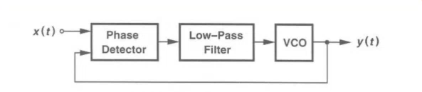
\includegraphics[scale=1.4]{PLLSchema.png} 
\caption{Schema a Blocchi PLL}
\label{fig:foo}
\end{figure}
~\begin{figure}[H]%Phase Detector
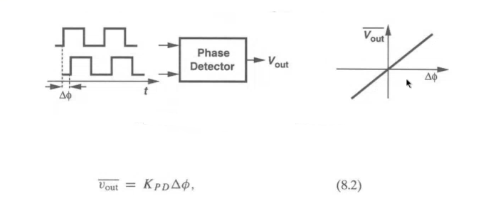
\includegraphics[scale=1]{PhaseDetect.png} 
\caption{Il Phase Detector lega la differenza di fase degli ingressi alla tensione d'uscita.}
\label{fig:foo}
\end{figure}




~\begin{figure}[!h]%Risposta al gradino
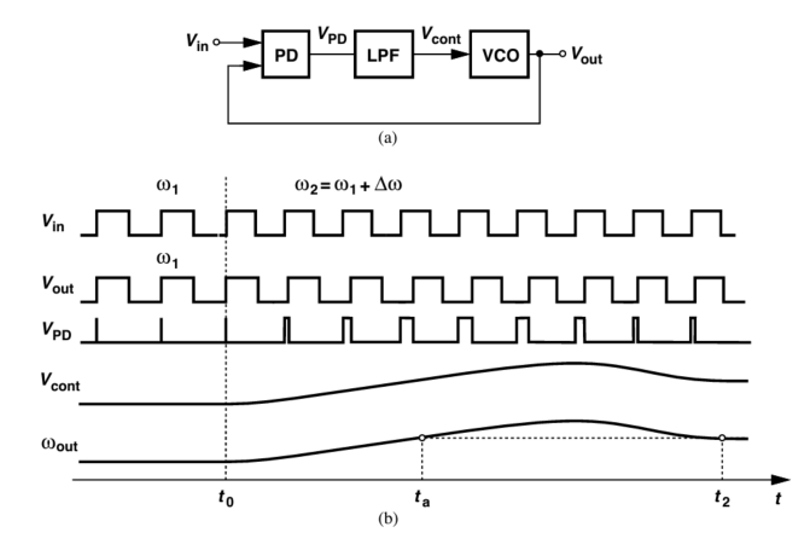
\includegraphics[scale=0.6]{PLLGradino.png} 
\caption{Risposta ad un gradino in frequenza}
\label{fig:foo}
\end{figure}
\paragraph{Analizzando la Figura 3, possiamo capire che se la tensione in uscita dal VCO è nulla (o al valore di riferimento), esso oscillerà ad una frequenza $\omega _{0}$, per modificare questa frequenza c'è necessità di cambiare la tensione di controllo $V_{CONT}$ in uscita dal LPF, la differenza di fase tra $V_{IN}$ e $V_{OUT}$ permette a $V_{PD}$ di generare un $\Delta V$ per modificare la frequenza del VCO. Il LPF deve "pulire" la tensione di controllo dai piccoli picchi che la tensione $V_{PD}$ avrebbe. 
Nell'istante $t_{0}$ la frequenza del segnale d'ingresso cambia, il periodo della Vin diminuisce, l'impulso VPD si allarga facendo aumentare $V_{CONT}$, all'istante $t_{a}$, a causa delle dinamiche dell'anello, la tensione $V_{CONT}$ continua a salire, facendo aumentare conseguentemente la frequenza di oscillazione del VCO, fino a quando non si stabilizzerà a $\omega _{1}$ all'istante $t_{2}$.\\Andando ad esplicitare il LPF come un filtro del primo ordine, otteniamo quanto segue in Figura 4}
~\begin{figure}[!h]%Risposta al gradino
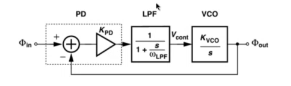
\includegraphics[scale=1.5]{Esplicitato.png} 
\caption{}
\label{fig:foo}
\end{figure}
\paragraph{Abbiamo la proporzionalità data dal PD, un polo dato dal LPF ed infine l'integratore che rappresenta il VCO. Possiamo calcolare le funzioni di trasferimento, sia ad anello aperto, sia ad anello chiuso ottenendo:\\$H_{0}(s)=K_{PD}\frac{1}{1+\frac{s}{\omega _{LPF}}}\frac{K_{VCO}}{s}$   e   $H(s)=\frac{K_{PD}K_{VCO}}{\frac{s^{2}}{\omega_{LPF}}}+s+K_{PD}K_{VCO}$}
\paragraph{Quanto detto fin'ora però presenta un problema: abbiamo\\ $\omega_{LPF}<<\omega_{IN}-\omega_{OUT}$, pertanto la differenza non riesce a passare nel LPF e il circuito non riesce ad agganciarsi. Per il nostro progetto quindi avremmo bisogno di un rivelatore che non tenga conto solo della fase ma anche della frequenza: PFD (Phase-Frequency Detector, Figura 5).}
~\begin{figure}[!h]%Risposta al gradino
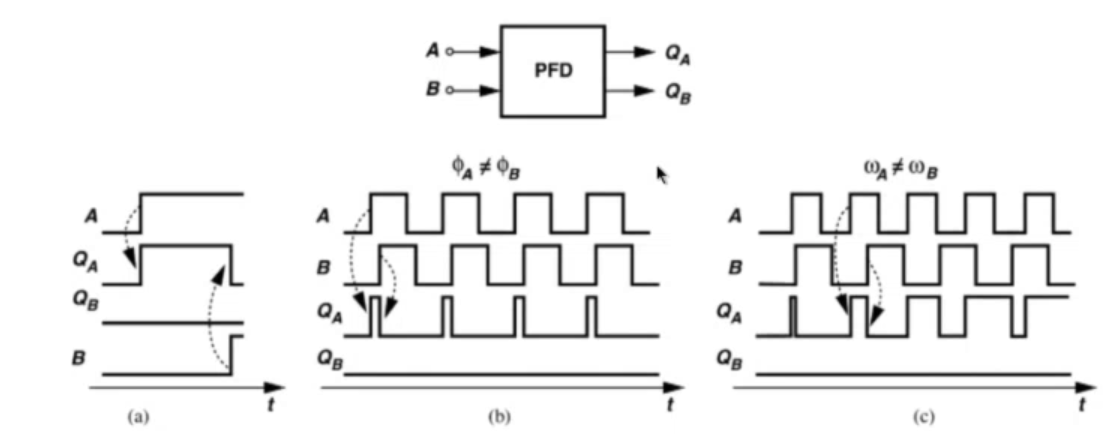
\includegraphics[scale=0.4]{PFD2.png} 
\centering
\caption{Schema di un PFD}
\label{fig:foo}
\end{figure}
\paragraph{\\\\Se il fronte di salita del segnale $A$ arriva prima del fronte del segnale $B$, il segnale d'uscita $Q_A$ va a 1 fino a quando non arriva il fronte di B, quindi la larghezza dell'impulso di $Q_A$ è proporzionale alla differenza di fase tra i due segnali. Al contrario ovviamente se $B$ fosse in anticipo rispetto ad $A$, accadrebbe la medesima cosa però sul segnale $Q_B$.
Questo dispositivo è stato implementato come si può vedere in Figura 6.
}
~\begin{figure}[!h]%Risposta al gradino
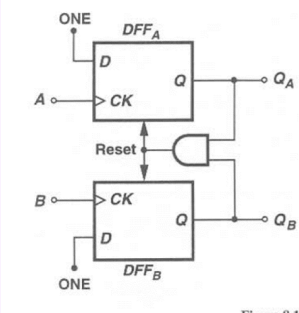
\includegraphics[scale=0.6]{PFD.png} 
\centering
\caption{Realizzazione di un PFD}
\label{fig:foo}
\end{figure}
\paragraph{A questo punto andiamo a realizzare un pompa di carico da aggiungere in cascata al PFD}
~\begin{figure}[!h]%Risposta al gradino
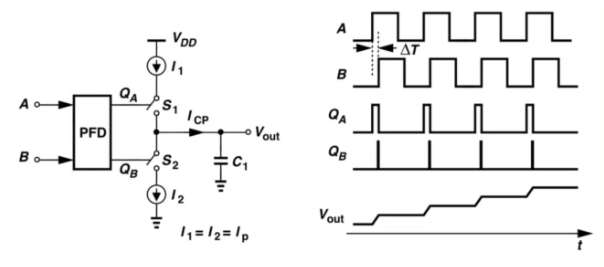
\includegraphics[scale=0.6]{CP.png} 
\caption{Rappresentazione simbolica della Charge Pump}
\label{fig:foo}
\end{figure}
\paragraph{Se $Q_A$ è a 1, chiude lo switch $S_1$, facendo caricare il condensatore $C_1$, facendo aumentare la frequenza del VCO.
L'uscita $Q_B$ invece fa scaricare lievemente il condensatore, in quanto gli impulsi di $Q_B$ sono molto più stretti di quelli di $Q_A$, il condensatore $C_1$ sostituisce anche il LPF, generando però un problema, la nuova funzione di trasferimento è $H(S)=\frac{I_PK_{VCO}}{2\pi C_1S^2+I_PK_{VCO}}$}

\paragraph{Questa presenta due poli immaginari nell'origine, rendendo così il sistema instabile. A questo punto per ovviare a questo problema si deve  aggiungere uno zero in zero alla funzione di trasferimento, aggiungendo un resistore prima del condensatore.
Il fattore di smorzamento diventa \textgreater 0 , il margine di fase, che in precedenza era nullo, ora è aumentato.  
Questo non è l'unico aspetto positivo di questa realizzazione, perché anche all'aumentare del guadagno, vediamo che il margine di fase aumenta ulteriormente di conseguenza (Figura 8), migliorando la stabilità.}
~\begin{figure}[!h]%Risposta al gradino
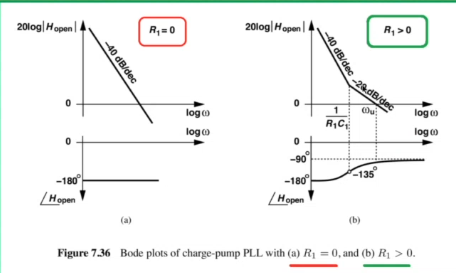
\includegraphics[scale=0.8]{ZPFD.png} 
\caption{Il margine di fase aumenta}
\label{fig:foo}
\end{figure}
\paragraph{Nella Figura 7 possiamo vedere che sarebbero necessari due generatori di corrente(ideali).
Ovviamente non possiamo avere dei generatori ideali, quindi approssimeremo i due generatori come due generatori reali, quindi con una $r_p$ in parallelo al generatore, che possiamo trasformarlo in un equivalente Thevenin quindi con la $r_p$ in serie.
A questo punto possiamo utilizzare due buffer Tristate, uno con ingresso a 1, l'altro con l'ingresso a 0. Collegando le due uscite $Q_A e Q_B$ del PFD agli input enable dei due buffer, avremo una approssimazione dei nostri due generatori (Figura 9). In serie alle due uscite dei buffer andremo poi ad inserire due resistenze $R_{P1}$ e  $R_{P2}$ che sarebbero quelle dei generatori reali.}
~\begin{figure}[!h]%Risposta al gradino
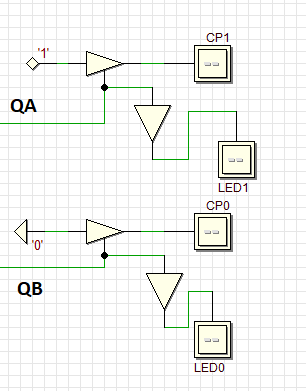
\includegraphics[scale=0.8]{CPDeeds.png} 
\centering
\caption{Realizzazione su Deeds dei due generatori di corrente}
\label{fig:foo}
\end{figure}
\paragraph{Il segnale $CP1$ e $CP2$ sono le uscite effettive della pompa di carico che andranno sul LPF, mentre le due uscite LED0 e LED1 sono state inserite per vedere i led della FPGA quando il nostro sistema sta modificando la frequenza di oscillazione. Ci sono infinite soluzioni per dimensionare i componenti necessari in questo blocco del nostro sistema, in questo caso $R_{P1}$ e  $R_{P2}$ sono state scelte pari a $27k\Omega$ quindi le correnti che scorrono nei due rami sono $I_1=I_2=\frac{V_{DD}-V{CONT}}{R_{P1}}$ essendo $V{CONT}=V_{DD}/2$ $I_1=I_2=60\mu A$. A questo punto dovremmo scegliere una $R_1$ (quella del LPF) di valore significativamente più bassa delle due appena scelte, pertanto scegliamo $R_1=\frac{R_{P1}}{10}=2.7k\Omega$.
Per dimensionare $C_1$ andremo a prendere la formula del fattore di smorzamento $\zeta$ che vedremo in seguito, dopo aver aggiunto il divisore per M, e lo porremo uguale a 0.8/1 che ci porterà alla stabilità del sistema. }
\paragraph{A questo punto possiamo inserire un divisore di frequenza.}
~\begin{figure}[!h]%Risposta al gradino
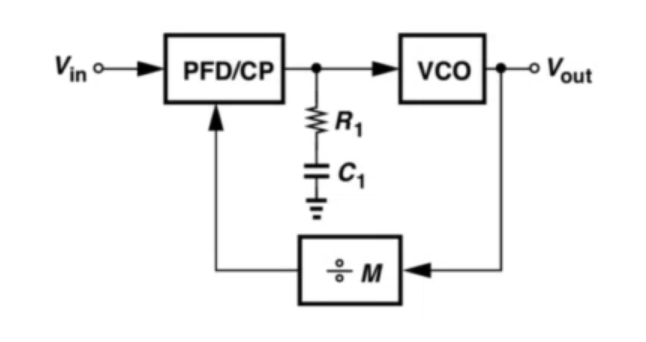
\includegraphics[scale=0.6]{DivM.png} 
\caption{PLL con pompa di carico e divisore per M}
\label{fig:foo}
\end{figure}
\paragraph{Il $K_{VCO}$ sarà noto in quanto parametro di costruzione.
Con l'inserimento del divisore per M abbiamo $\omega _n=\sqrt{\frac{I_p K_{VCO}}{2 \pi C_1M} }$ e $\zeta=\frac{R_1}{2}\sqrt{\frac{I_p K_{VCO}C_1}{2\pi M}}$ a questo punto possiamo andare a dimensionare $C_1$ sapendo che\\ $\zeta \approx0.8 \div 1$, $K_{VCO}\approx800$ per $C_{EXT}=120pF$, $I_P=60\mu A$ e $M=100$.
Ponendo $\zeta \approx0.94$ otteniamo una capacità $C_1=1\mu F$  }
 

\paragraph{Per il nostro progetto dovremo tenere conto delle richieste che sono:\\$f_{OUT}=1 MHz$\\$f_{REF}=10 kHz$\\$M=100 (80\div150)$.\\Il VCO che utilizzeremo sarà il 74LS624, sono presenti due alimentazioni separate, una per la parte logica ed una per la parte di oscillazione, perché il costruttore ci dice che per frequenze \textgreater 10MHz è consigliato l'utilizzo di alimentazioni separate, in modo tale che i rumori proveniente dalla parte logica non influiscano sulla frequenza di oscillazione, infatti se la tensione di alimentazione avesse delle lievi oscillazioni la frequenza di lavoro cambierebbe.
Tuttavia, nel nostro caso, utilizzeremo una singola alimentazione.}
~\begin{figure}[!h]%Risposta al gradino
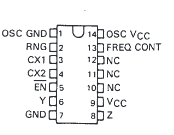
\includegraphics[scale=1]{74LS.png} 
\centering
\caption{Pinout del VCO}
\label{fig:foo}
\end{figure}
\paragraph{Come si diceva prima, si vedono infatti i pin delle due alimentazioni separate(1-14, 7-9), il piedino di enable, nel nostro caso, lo lasciamo sempre collegato a GND per farlo lavorare ogni volta che il VCO è alimentato.
Il piedino 13 è quello di ingresso della tensione di controllo che proviene da un buffer, il motivo per cui è stato inserito un buffer tra il LPF e il VCO è che dal piedino di input ci sono delle resistenze che potrebbero costituire un carico non trascurabile, pertanto inserendo un buffer realizzato con un amplificatore operazionale andremo ad ovviare a questo problema.\\I pin 3 e 4 sono per una capacità esterna che noi abbiamo preso $C_{EXT}=120pF$.}
~\begin{figure}[!h]%Risposta al gradino
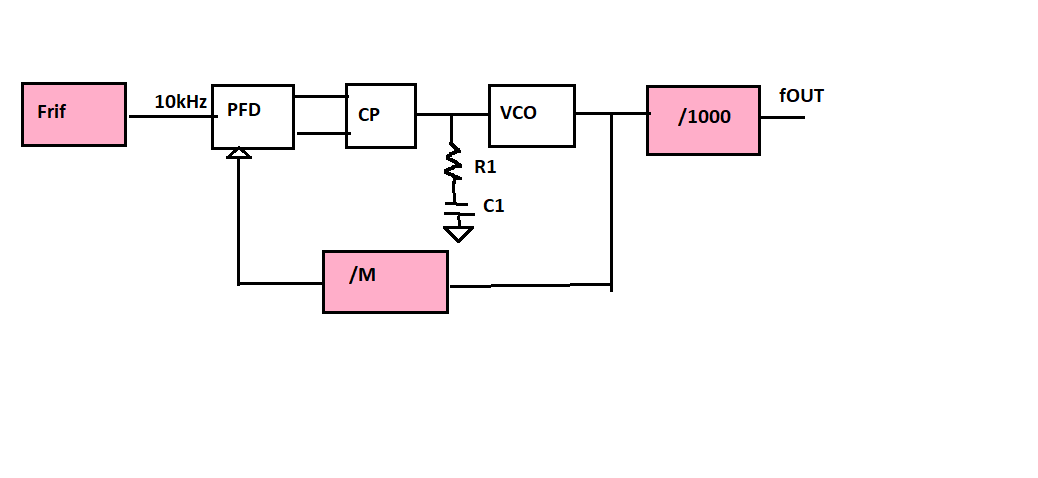
\includegraphics[scale=0.4]{SCH.png} 
\centering
\caption{Schema a blocchi dei dispositivi da realizzare.}
\label{fig:foo}
\end{figure}
\paragraph{Il divisore per M, realizzato sull'FPGA, presenterà uno dip switch, da 8 interruttori, per selezionare il numero M. Il DIP switch verrà collegato a due array di resistenze, quando uno singolo switch sarà ON, l'ingresso sulla FPGA verrà visto come basso, perché collegato a massa(attraverso le due resistenze), mentre, se lo switch è su OFF, l'ingresso della FPGA vede il valore logico alto (3.3V).}
\paragraph{A questo punto l'uscita del VCO avrà un'uscita massima \textgreater 4V e dobbiamo portarlo in un range tale da poterlo usare come ingresso al divisore, quindi alla FPGA, per cui dobbiamo utilizzare un Level Shifter per portarlo a 3.3V.}
~\begin{figure}[!h]%Risposta al gradino
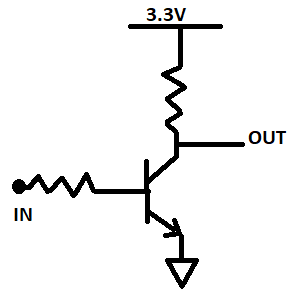
\includegraphics[scale=0.7]{Level.png} 
\centering
\caption{Level Shifter}
\label{fig:foo}
\end{figure}
\paragraph{Lo scopo di questo blocco è quindi quello di traslare il livello logico 1 dal valore che ci dava il VCO (\textgreater 4V) a 3.3V, mediante l'utilizzo di un transistore NPN 2N2222 (o similare), la resistenza di pull-up è stata scelta da $1.5k\Omega$ e quella in serie all'ingresso è stata presa da $15k\Omega$.\\
Lo schema a blocchi completo di ogni componente è quindi il seguente:}
~\begin{figure}[!h]%Risposta al gradino
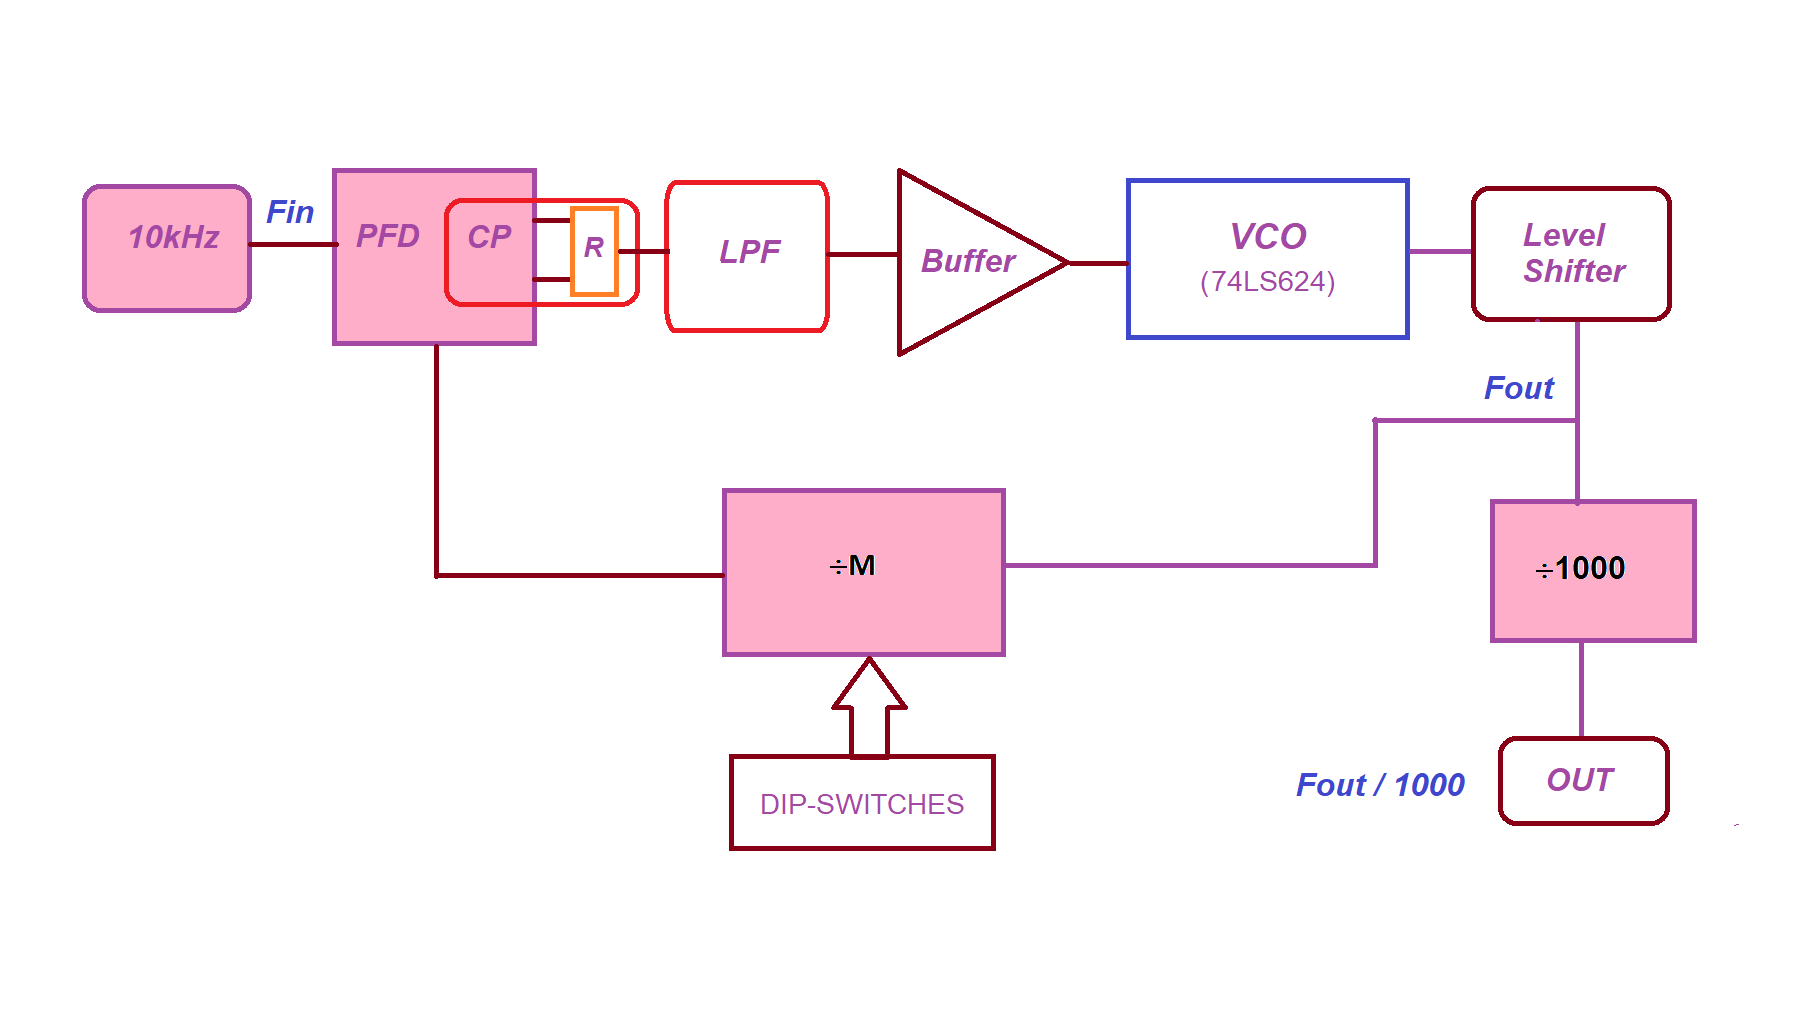
\includegraphics[scale=0.4]{PLL_1.png} 
\centering
\caption{Schema a blocchi completo}
\label{fig:foo}
\end{figure}


\newpage
\section{Realizzazione}
La realizzazione pratica è quindi suddivisa in due step, il primo su Deeds ed il secondo su breadboard.
\subsection{Parte su Deeds}
\paragraph{La prima cosa fatta per realizzare il sintetizzatore è stata partire dall'implementare sul Digital Electronics Deeds tutte le componenti che dovranno poi essere messe sulla FPGA Cyclone II.}
~\begin{figure}[!h]%Risposta al gradino
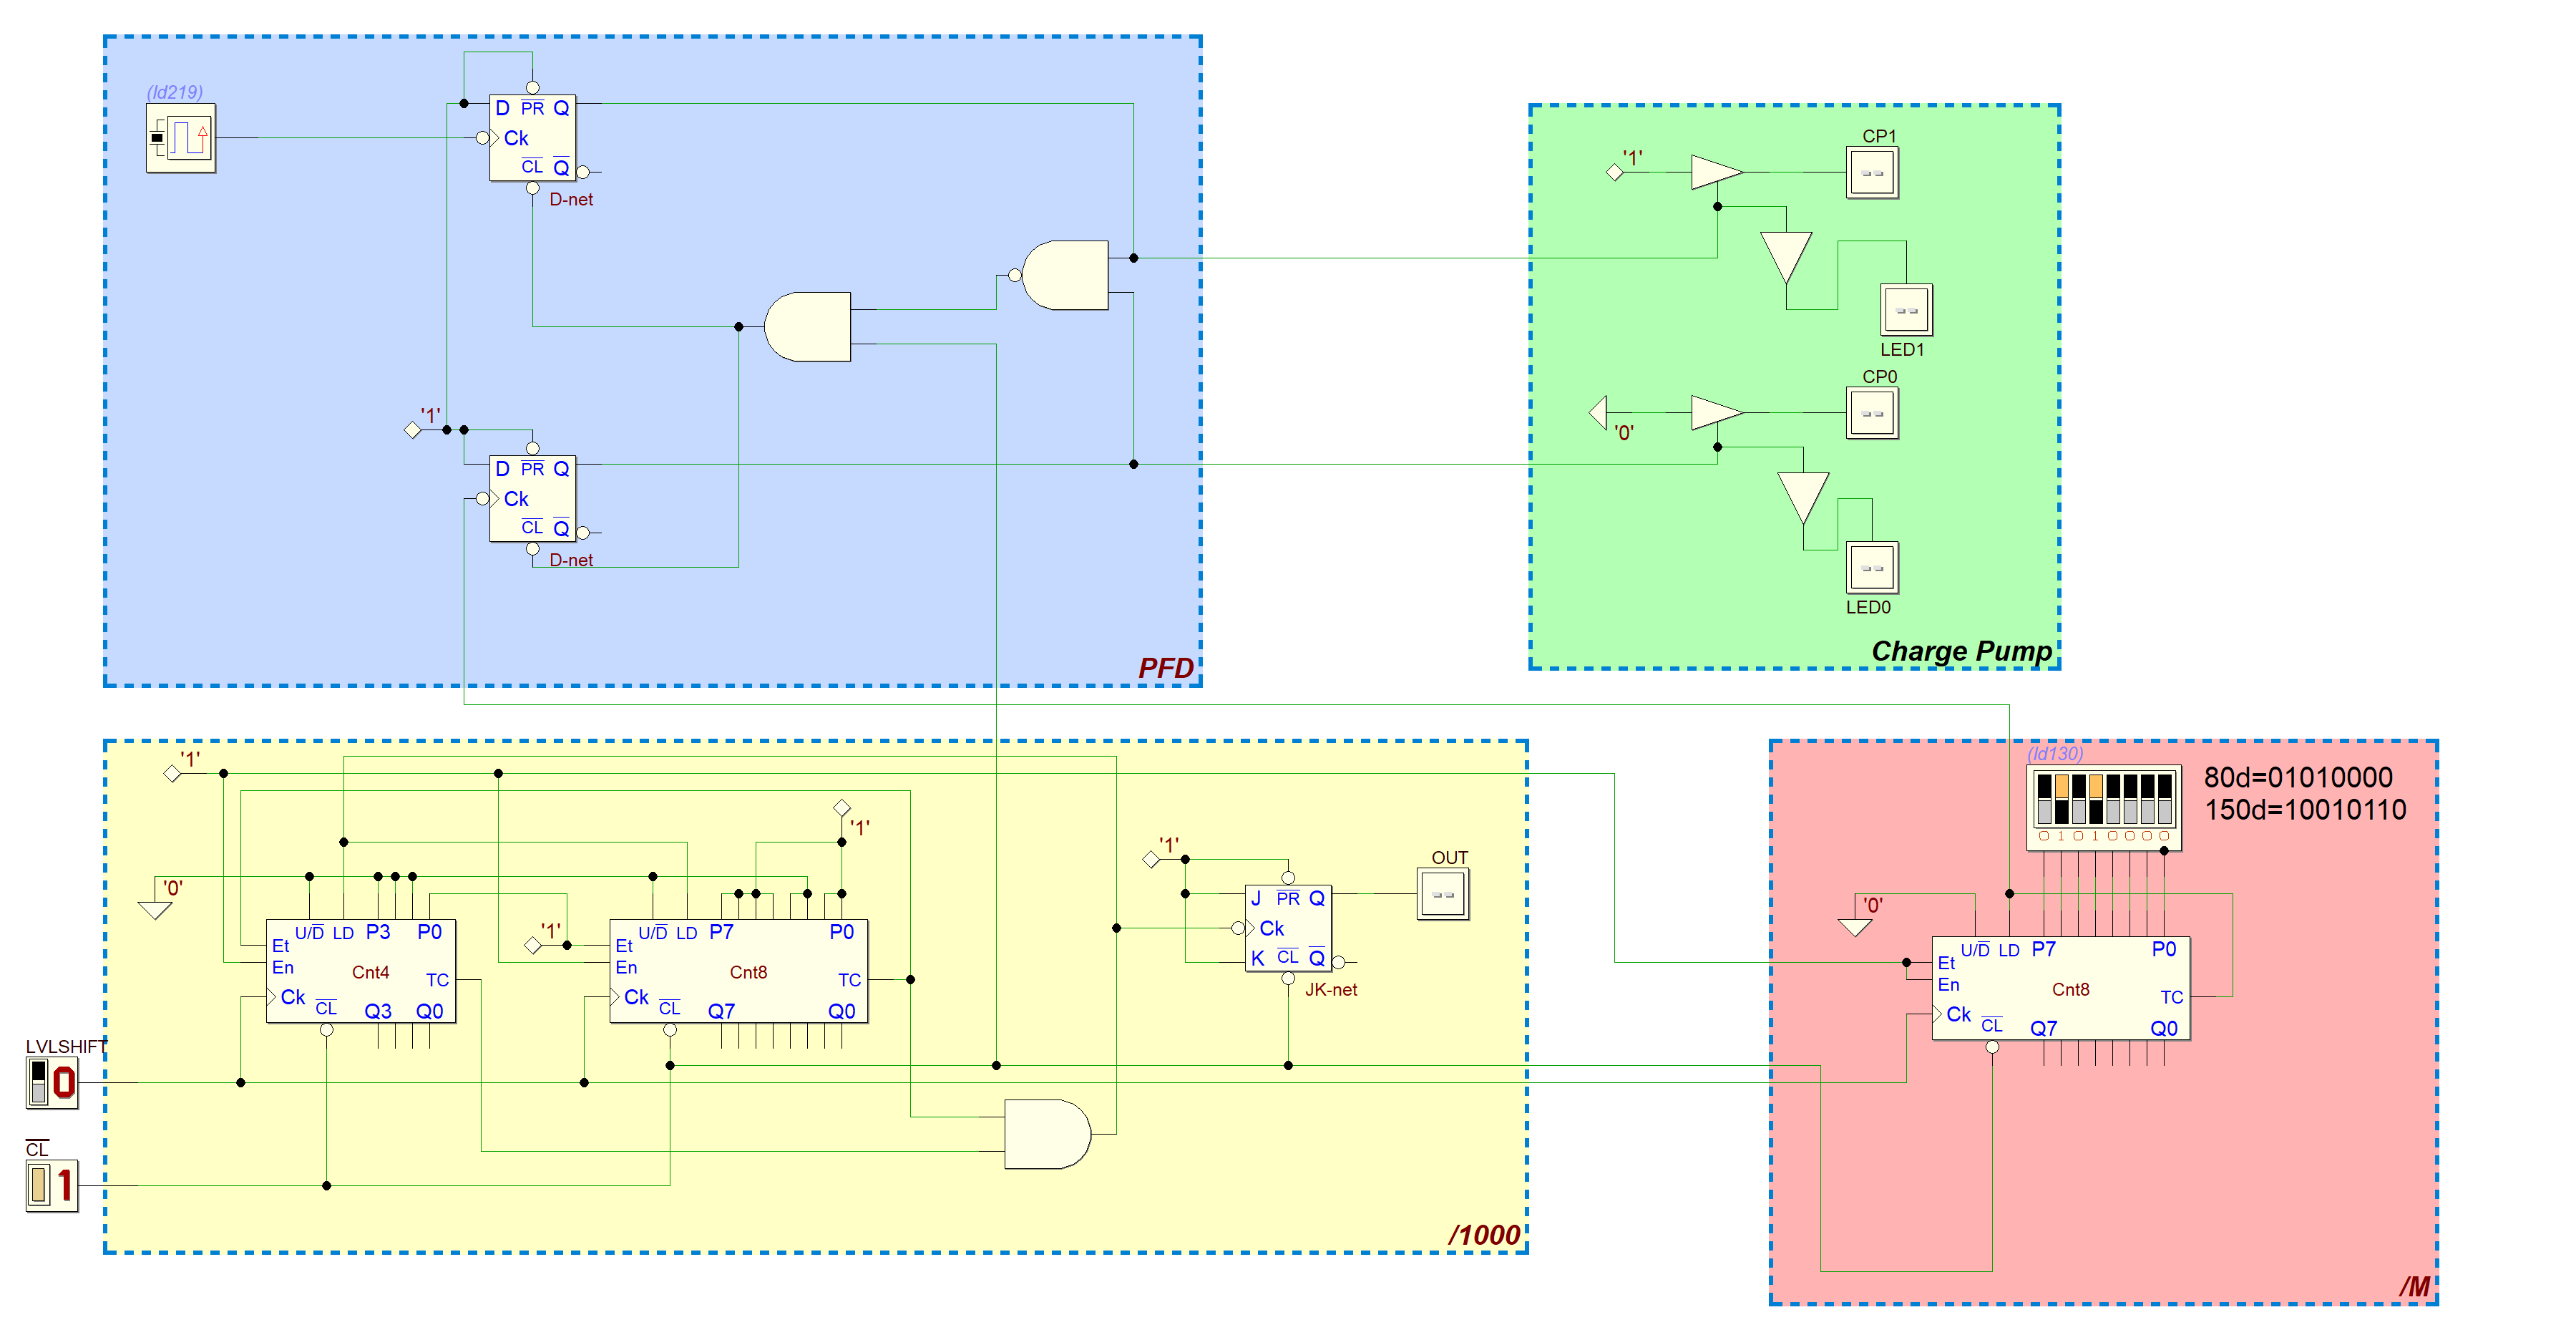
\includegraphics[scale=4.4]{Fig_Finale.png} 
\centering
\caption{Schema realizzato su Deeds}
\label{fig:foo}
\end{figure}
\paragraph{In azzurro c'è il rilevatore di frequenza e fase, le cui uscite vanno alla pompa di carica (in verde).\\In Giallo e in rosso possiamo vedere i due divisori, realizzati con due contatori.
A sinistra c'è il divisore per mille, realizzato caricando il numero $000111110011$ ovvero 499, siccome conta fino a zero, impiegano 500 cicli di clock per arrivare a zero, il filp-flop JK nella configurazione in figura ha il compito di dividere ulteriormente a metà la frequenza, ottenendo così il desiderato divisore per mille.\\
Con lo stesso principio, in rosso, abbiamo il divisore per M variabile, il numero M viene scelto mediante gli switch in alto.
L'ingresso di entrambi i divisori è ovviamente l'uscita del level shifter realizzato su breadboard come spiegato nel capitolo precedente.\\L'uscita finale è l'uscita Q del Flip Flop JK e il clock in alto a sinistra è la frequenza di riferimento.\\Mediante il software Quartus II, il progetto è stato esportato sulla FPGA, assegnando ad ogni Ingresso/uscita utile un suo pin da collegare poi alla breadboard.}
 \subsection{Parte su bread-board}
 \paragraph{Per il nostro progetto c'era bisogno di interfacciare la parte software con quella hardware, come detto prima sono stati assegnati i pin della FPGA nel modo seguente:}
 ~\begin{figure}[!h]%Risposta al gradino
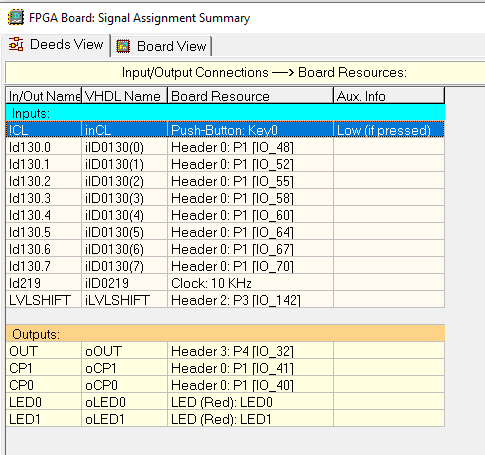
\includegraphics[scale=0.6]{PinDeeds.png} 
\centering
\caption{Assegnazione dei pin}
\label{fig:foo}
\end{figure}
\paragraph{Il clear è stato messo sul push button della FPGA, i PIN dal 48 al 70 sono stati usati per collegare i dip switches alla FPGA, e l'uscita del level shifter (che andrà ai due divisori) è stato assegnato al pin 142. Su ogni componente sono stati messi dei condensatori di bypass sulle alimentazioni per ridurre al minimo le oscillazioni che la tensione di alimentazione potrebbe avere.
Lo schema del circuito realizzato su breadboard è il seguente:}
 ~\begin{figure}[!h]%Risposta al gradino
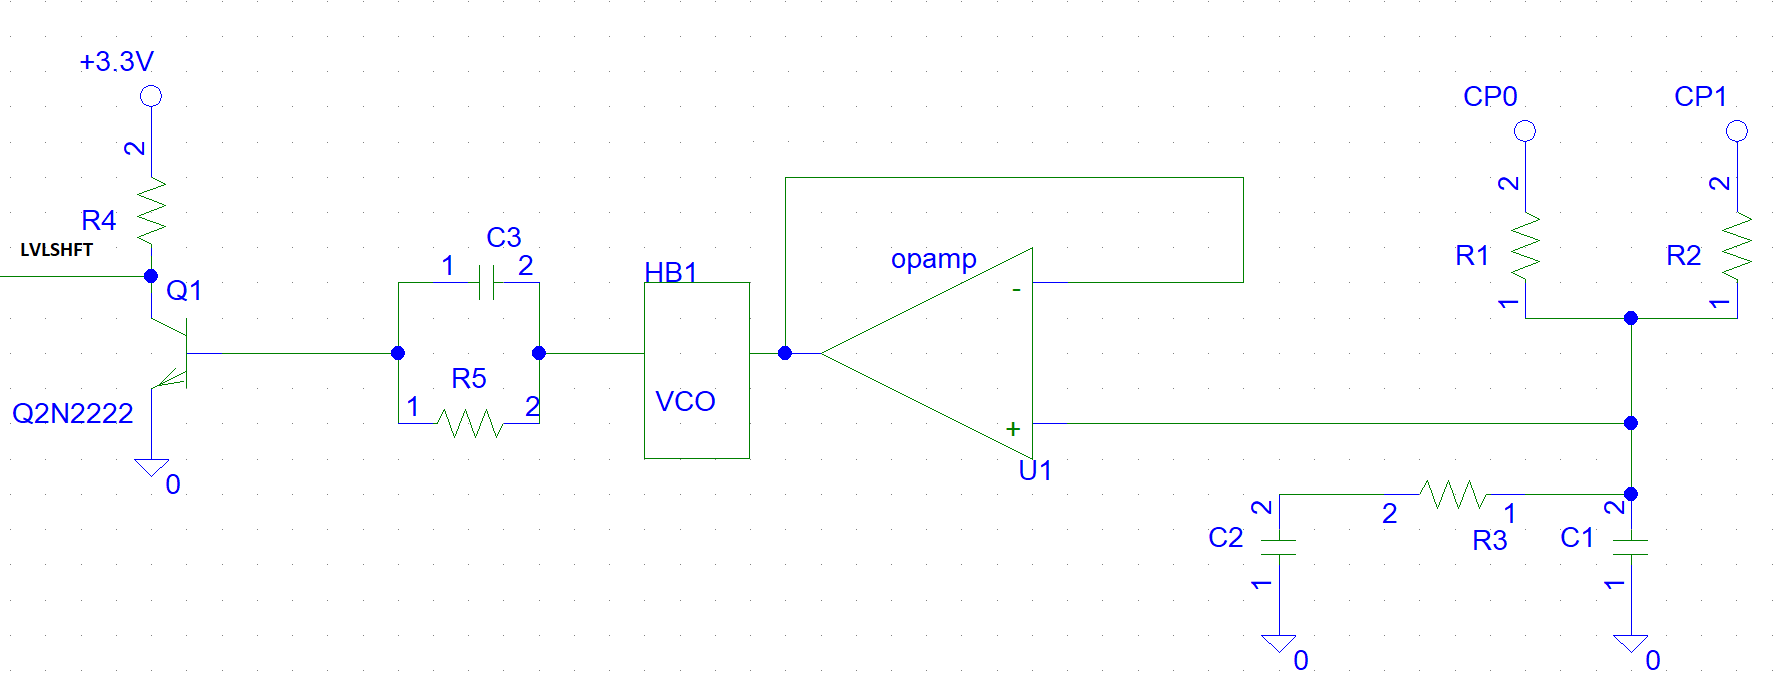
\includegraphics[scale=0.35]{SchemaCirc.png} 
\centering
\caption{Schema circuitale realizzato}
\label{fig:foo}
\end{figure}

 ~\begin{figure}[!h]%Risposta al gradino
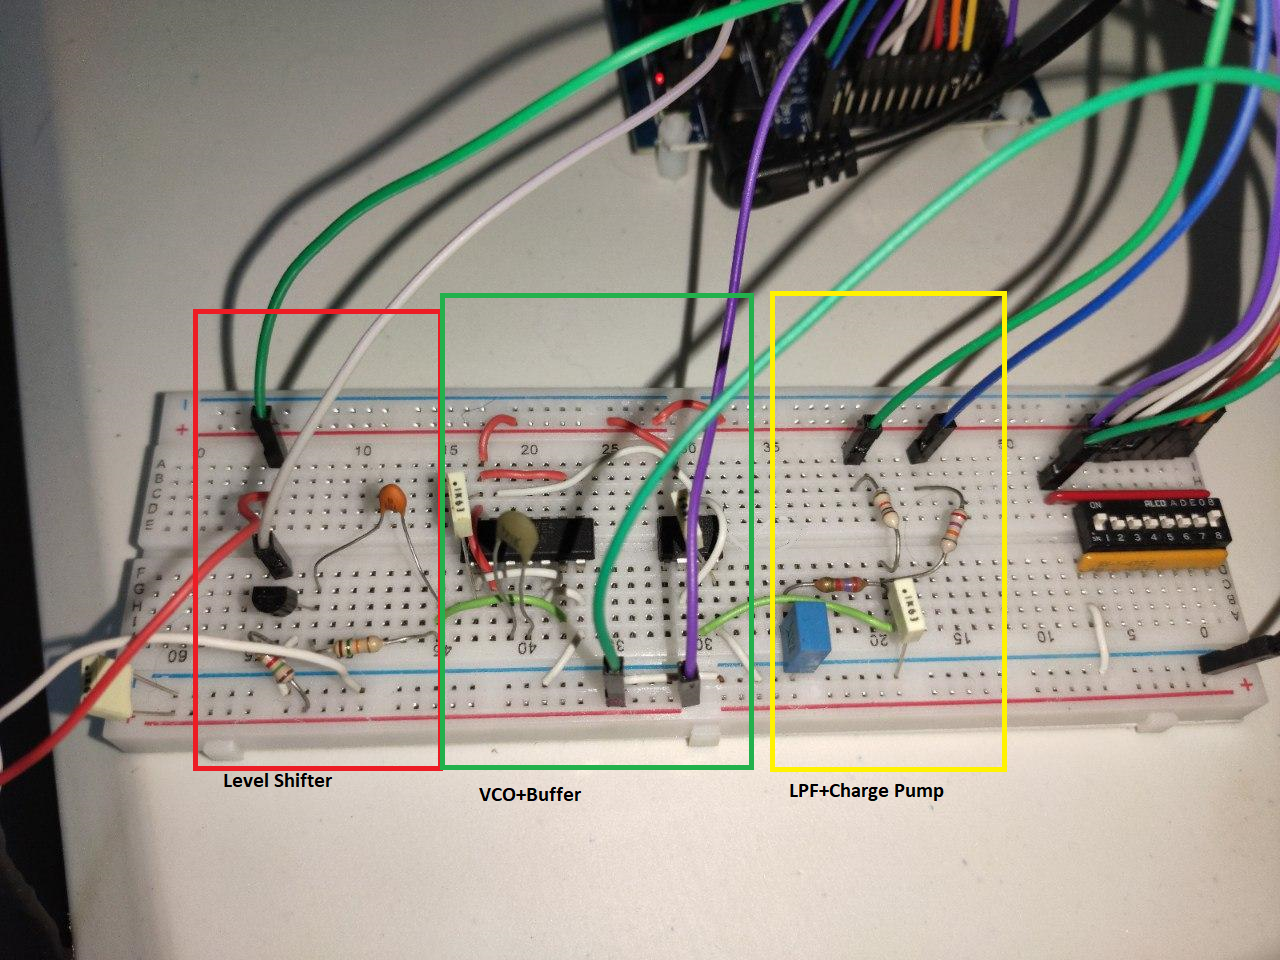
\includegraphics[scale=0.3]{Circuito.png} 
\centering
\caption{Realizzazione Pratica}
\label{fig:foo}
\end{figure}
\newpage
\section{Risultati}
\paragraph{Per visualizzare l'onda d'uscita si è utilizzato il software SoundScope che, interfacciandosi con la scheda audio del computer, mostra la forma d'onda in ingresso sul canale microfono. Di seguito vengono riportati diverse uscite al variare di M}
\subsection{Screenshot dell'oscilloscopio}

\begin{figure}[H]
   \begin{minipage}{0.48\textwidth}
     \centering
     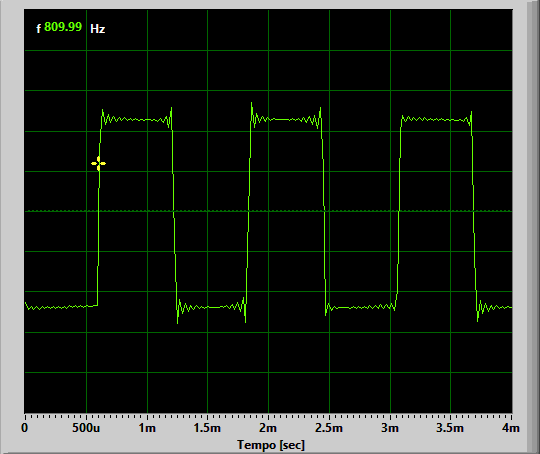
\includegraphics[width=1\linewidth]{m80}
     \caption{M=80 - Dominio del tempo}\label{Fig:Data1}
   \end{minipage}\hfill
   \begin{minipage}{0.48\textwidth}
     \centering
     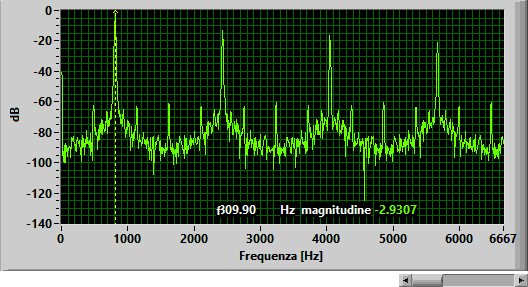
\includegraphics[width=1\linewidth]{m80f}
     \caption{M=80 - Dominio delle frequenze}\label{Fig:Data2}
   \end{minipage}
\end{figure}

\begin{figure}[H]
   \begin{minipage}{0.48\textwidth}
     \centering
     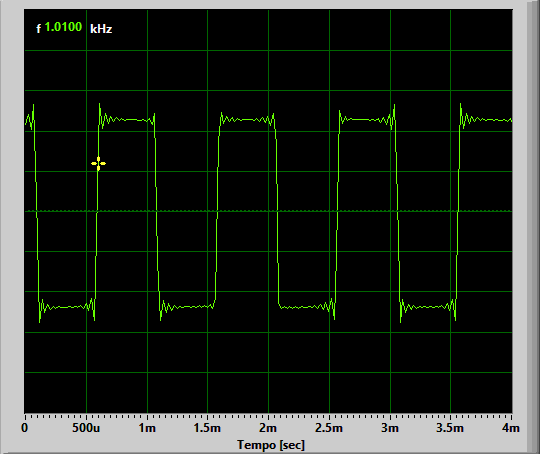
\includegraphics[width=1\linewidth]{m100}
     \caption{M=100 - Dominio del tempo}\label{Fig:Data1}
   \end{minipage}\hfill
   \begin{minipage}{0.48\textwidth}
     \centering
     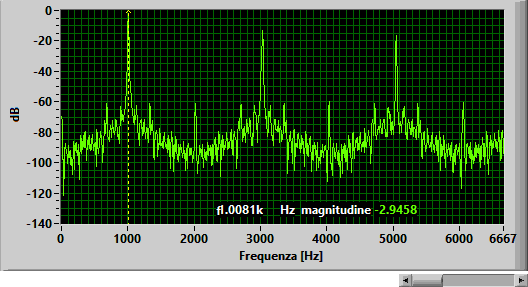
\includegraphics[width=1\linewidth]{m100f}
     \caption{M=100 - Dominio delle frequenze}\label{Fig:Data2}
   \end{minipage}
\end{figure}
\begin{figure}[H]
   \begin{minipage}{0.48\textwidth}
     \centering
     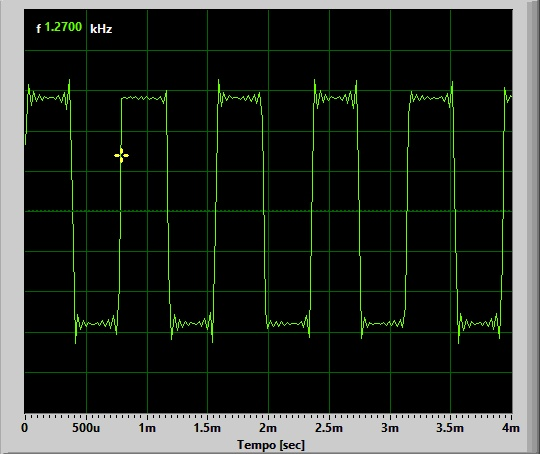
\includegraphics[width=1\linewidth]{m126}
     \caption{M=126 - Dominio del tempo}\label{Fig:Data1}
   \end{minipage}\hfill
   \begin{minipage}{0.48\textwidth}
     \centering
     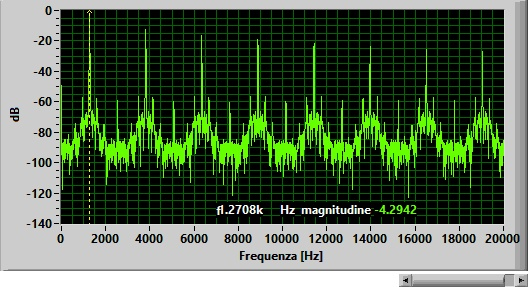
\includegraphics[width=1\linewidth]{m126f}
     \caption{M=126 - Dominio delle frequenze}\label{Fig:Data2}
   \end{minipage}
\end{figure}



\section{Conclusioni}
\paragraph{Per concludere, si è prima realizzata la parte su FPGA e verificato il suo corretto sviluppo mediante test con segnali noti, solo in seguito è stata realizzata la parte su bread-board dopo aver opportunamente dimensionato i componenti(vedi capitolo 2).
Si è utilizzato il software SoundScope per visualizzare a schermo l'onda d'uscita, la frequenza e l'analisi spettrale.}

\newpage
\section{Riferimenti}
\paragraph{Alcune immagini e schemi circuitali sono stati presi da: }
\begin{itemize}
\item Design of CMOS Phase-Locked Loops - B. Razavi
\item RF Microelectronics - B. Razavi
\end{itemize}
\end{document}
